\subsection*{Magnetic Field Generation}

Magnetic fields were generated using a \textbf{custom-built air-core solenoid}, approximately 15 cm in length and 10 cm in outer diameter. The solenoid was densely wound with \textbf{copper wire ($\sim$1 mm diameter)}, forming an inner core of approximately 5 cm. A \textbf{Pasco Scientific SF-9584 DC power supply} was used to deliver currents in the range of \textbf{0--4 A}, corresponding to magnetic field strengths from \textbf{1 to 18.9 Gauss}. The system operated in a continuous mode; no rest periods were applied between trials due to the time required to stabilize the pendulum after each adjustment. Figure \ref{labsetup} shows the experimental lab setup used to assess the methodology accuracy and reliability with all used components.

%figure from pptx

\begin{figure}[H]
	\centering
	\begin{minipage}[t]{0.58\textwidth}
		\centering
		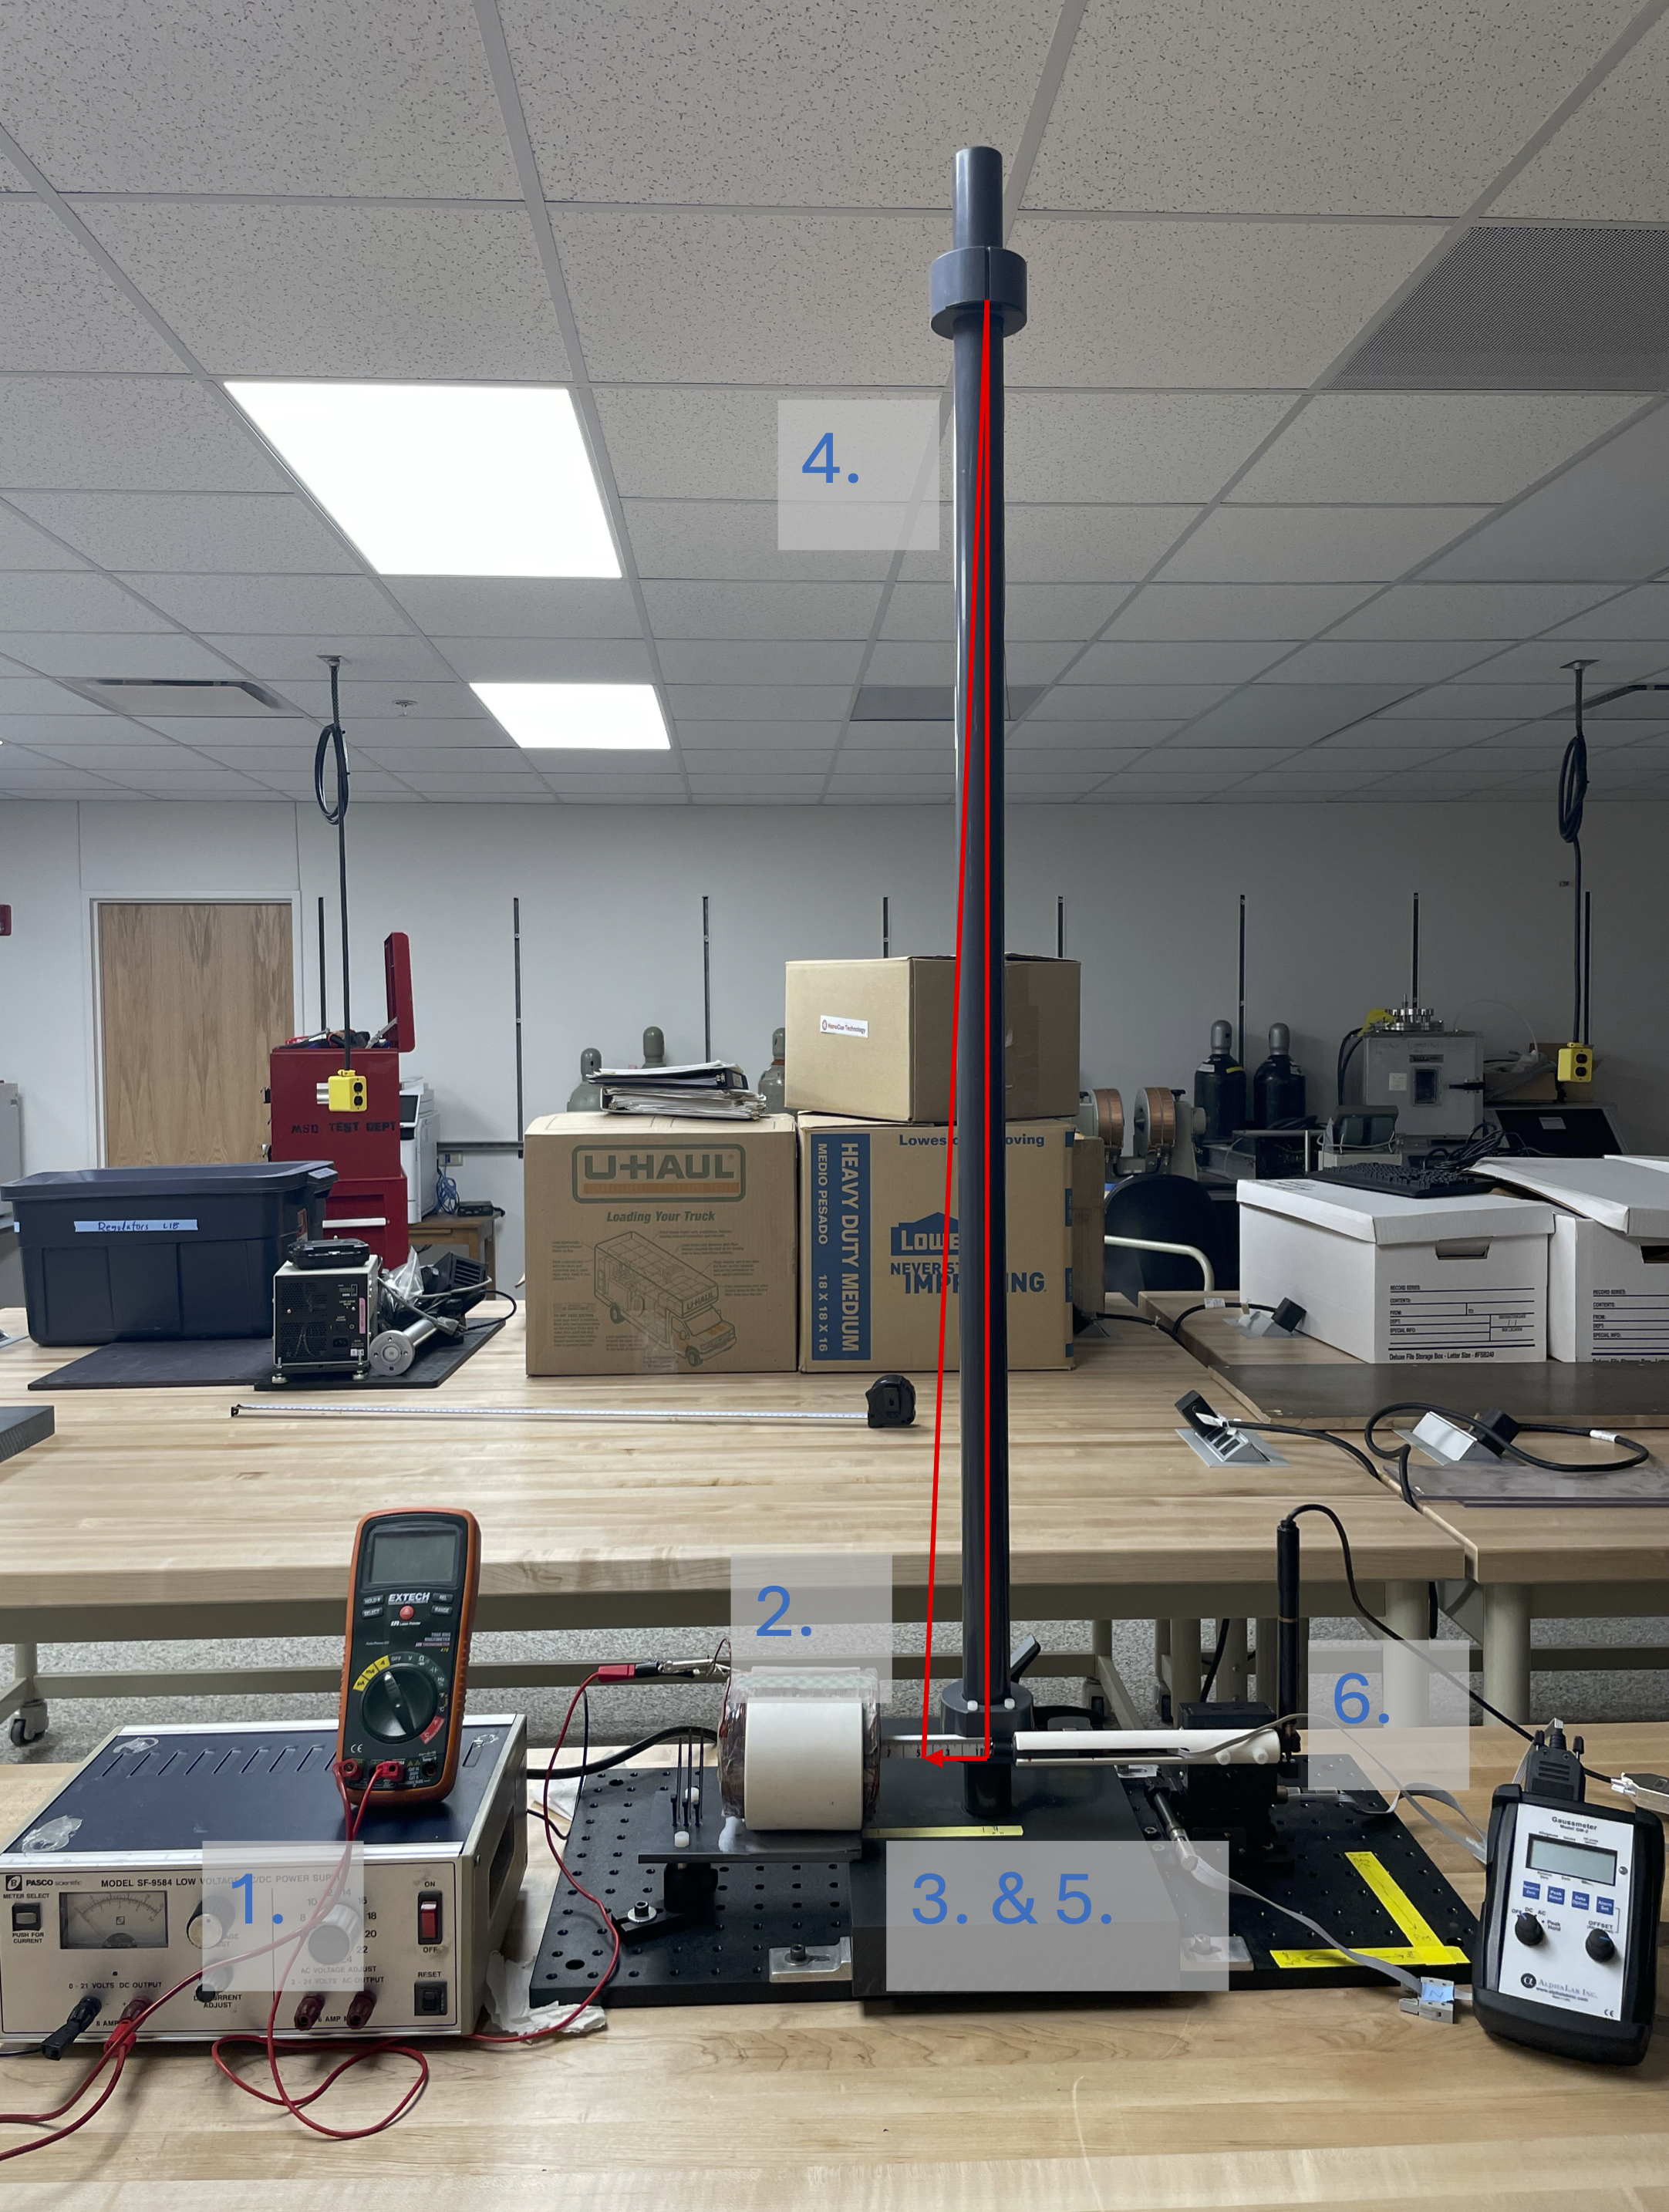
\includegraphics[width=\textwidth]{Assests/labsetup.png} % Update with the labeled version if needed
	\end{minipage}%
	\hfill
	\begin{minipage}[t]{0.42\textwidth}
		\footnotesize
		\vspace*{-50ex}
		\begin{enumerate}
			\item Power Supply with Ammeter $\pm$ .001 A 
			\item Solenoid (1 to 20 Gauss)
			\item Ruler (Deflection Angle) $\pm$1 mm 
			\item PVC String Pole
			\item Ferromagnetic Cylinder
			\item AlphaLab, Inc. Gaussmeter $\pm$0.001 G  
		\end{enumerate}
	\end{minipage}
	\caption{In-lab experimental setup for MRI translational force assessment. Labeled components include the solenoid, pendulum fixture, measurement tools, and control equipment.}
	\label{labsetup}
\end{figure}

LABVIEW program and Alpha Labs Protocols


\subsection{Magnetic Field and Gradient Mapping Platform}

Magnetic field strength ($B_0$) and gradient ($\nabla B_0$) measurements were performed using a commercial Hall-effect Gaussmeter (Model GM2, AlphaLab Inc., Salt Lake City, UT).  The GM2 operates on the Hall effect principle, wherein a voltage is generated across a probe when exposed to a perpendicular magnetic field. This voltage is proportional to the local magnetic flux density, enabling precise spot measurements of field magnitude. The Gaussmeter used has an accuracy of 1\% of the DC reading in the 16$^\circ$C to 29$^\circ$C range.

To ensure spatial accuracy and reproducibility, a fixture made from rigid \gls{pvc} was constructed by previous Creighton University students \cite{haddixProposal}. The platform comprises a 300 mm square base and a 280 mm diameter vertical circular plate, perforated with a 5x5 grid of probe-access holes spaced at 20 mm intervals as shown in figure \ref{fig:fieldmapping}. Each access point was numerically indexed to facilitate 2D field mapping in the X-Y plane.

In clinical use, the entire fixture is intended to be shifted axially along the Z-direction of a horizontal bore MRI scanner using controlled couch increments (e.g., 10 cm). This translation allows for volumetric sampling of $B_0$ over several planes. The spatial magnetic field gradient$\nabla B_0$ can then be estimated numerically using finite difference calculations between adjacent measurement points. This method has previously been applied to MRI mapping in the work by Ferreira \cite{ferreira2017}.

\begin{figure}[H]
	\centering
	\includegraphics[width=0.5\textwidth]{Assests/Picture3.jpg}
	\caption{PVC-based magnetic field mapping platform used for spatial $B_0$ and $\nabla B_0$ measurement. As shown in Ferreira 2017 \cite{haddixProposal,ferreira2017}}
	\label{fig:fieldmapping}
\end{figure}

